\documentclass[letterpaper]{article}
\usepackage{amssymb}
\usepackage{fullpage}
\usepackage{changepage}
\usepackage{amsmath}
\usepackage{epsfig,float,alltt}
\usepackage{psfrag,xr}
\usepackage[T1]{fontenc}
\usepackage{url}
\usepackage{pdfpages}
\usepackage{epstopdf}
\usepackage[framed,numbered,autolinebreaks,useliterate]{mcode}

%\includepdfset{pagecommand=\thispagestyle{fancy}}
\author{Yi Yang}
\title{EECS 442 Homework \#2}

\begin{document}
\date{09/29/2016}
\maketitle

\newcommand{\trace}{\mathrm{trace}}
\newcommand{\real}{\mathbb R}  % real numbers  {I\!\!R}
\newcommand{\nat}{\mathbb N}   % Natural numbers {I\!\!N}
\newcommand{\cp}{\mathbb C}    % complex numbers  {I\!\!\!\!C}
\newcommand{\ds}{\displaystyle}
\newcommand{\mf}[2]{\frac{\ds #1}{\ds #2}}
\newcommand{\spanof}[1]{\textrm{span} \{ #1 \}}
\newcommand{\sol}[0]{\textbf{Solution: }}
\newcommand{\pf}[0]{\textbf{Proof:}}
\newcommand{\rme}[0]{\textrm{e}}
\newcommand{\Null}[1]{\textrm{Null}\{#1\}}
\parindent 0pt
%%%%%%%%%%%%%%%%%%%%%%%%%%%%%%%%%%%%%%%%%%%%%%%%%%%%%%%%%%%%%%%%%%%%%%%%%%%%%%%
% Solution for Question 1 begins here - by Yi Yang
%%%%%%%%%%%%%%%%%%%%%%%%%%%%%%%%%%%%%%%%%%%%%%%%%%%%%%%%%%%%%%%%%%%%%%%%%%%%%%%
\section*{Problem 1}
\subsection*{(a)}
Suppose there exists matrix $H_1$, $H_2$ and $H = H_1 H_2$ such that $\hat{M} = MH$, $\hat{M'} = M'H$. If we can solve for $H_1$ and $H_2$ respectively, then we can prove the statement is correct.
Consider:
$$H_1 = 
\begin{bmatrix}
A^{-1} & -A^{-1}b\\
0 & 1
\end{bmatrix}
\Rightarrow\quad MH_1 = 
\begin{bmatrix}
I & 0
\end{bmatrix}
, \quad	
M'H_1 = 
\begin{bmatrix}
A'A^{-1} & -A'A^{-1}b + b'
\end{bmatrix}
$$
Suppose the general form of $H_2$ is:
$$H_2 = 
\begin{bmatrix}
W_{3\times 3} & X_{3\times 1}\\
Y_{1\times 3} & Z_{1\times 1}
\end{bmatrix}
$$
Since
$$MH_1H_2 = 
\begin{bmatrix}
I & 0
\end{bmatrix}
\quad
M'H_1H_2 = 
\begin{bmatrix}
P_{2\times 3} & Q_{2\times 1}\\
0 & 1
\end{bmatrix}
$$
We can have:
$$W_{3\times 3} = I \quad X_{3\times 1} = 0$$
Hence, we need to prove the following relations:
$$M'H_1H_2 = 
\begin{bmatrix}
A'A^{-1} & -A'A^{-1}b + b'
\end{bmatrix}
\begin{bmatrix}
I & 0\\
Y_{1\times 3} & Z_{1\times 1}
\end{bmatrix} = 
\begin{bmatrix}
P_{2\times 3}& Q_{2\times 1}\\
0 & 1
\end{bmatrix}
$$
If we represent the elements of $M'H_1H_2$ as $n_{ij}$, then we can deduce the following equation:
$$\begin{bmatrix}
n_{3\times 1} & n_{3\times 2} & n_{3\times 3} & n_{3\times 4}
\end{bmatrix}
\begin{bmatrix}
I & 0\\
Y_{1\times 3} & Z_{1\times 1}
\end{bmatrix} = 
\begin{bmatrix}
P_{2\times 3} & Q_{2\times 1}\\
0 & 1
\end{bmatrix}
$$
Since we have the following relations:
$$e_{3}^T\left(-A'A^{-1}b + b'\right) \neq 0$$
Hence, we know that $n_{3\times 4} \neq 0$, and we can formulate $H_2$ as:
$$H_2 = 
\begin{bmatrix}
1 & 0 & 0 & 0\\
0 & 1 & 0 & 0\\
0 & 0 & 1 & 0\\
-\tfrac{n_{31}}{n_{34}} & -\tfrac{n_{32}}{n_{34}} & -\tfrac{n_{33}}{n_{34}} & \tfrac{1}{n_{34}}
\end{bmatrix}
$$
According to the derivation above, we know if we set $H = H_1H_2$, we will transform $M$ and $M'$ to $\hat{M}$ and $\hat{M'}$ respectively.

\subsection*{(b)}
It is obvious that
$$MX = \left(MH\right)\left(H^{-1}X\right)$$
$$M'X = \left(M'H\right)\left(H^{-1}X\right)$$
Hence, if $x$ and $x'$ are matched points with respect to the pair of cameras $\left(M, M'\right)$, corresponding to a 3D point, then they are also matched points with respect to the pair of cameras $\left(MH, M'H\right)$, corresponding to the point $H^{-1}X$, that is the fundamental matrix corresponding to two pairs are the same.
\subsection*{(c)}
According to the conclusions drawn from (b), we know the fundamental matrix corresponding to pair $(M,\; M')$ and $(\hat{M},\; \hat{M'})$ are the same, which is$[b]_xA$, that is:
$$F = [b]_xA = 
\begin{bmatrix}
0 & -1 & b_2\\
1 & 0 & -b_1\\
-b_2 & b_1 & 1
\end{bmatrix}
\begin{bmatrix}
a_{11} & a_{12} & a_{13}\\
a_{21} & a_{22} & a_{23}\\
0 & 0 & 0
\end{bmatrix}
= 
\begin{bmatrix}
-a_{21} & -a_{22} & -a_{23}\\
a_{11} & a_{12} & a_{13}\\
-b_2a_{11} + b_1a_{21} & -b_2a_{12} + b_1a_{22} & -b_2a_{13} + b_1a_{23}
\end{bmatrix}
$$
Hence, 
$$F = 
a_{12}
\begin{bmatrix}
-\mf{a_{21}}{a_{12}} & -\mf{a_{22}}{a_{12}} & -\mf{a_{23}}{a_{12}}\\
\mf{a_{11}}{a_{12}} & 1 & \mf{a_{13}}{a_{12}}\\
-b_2\mf{a_{11}}{a_{12}} + b_1\mf{a_{21}}{a_{12}} & -b_2 + b_1\mf{a_{22}}{a_{12}} & -b_2\mf{a_{13}}{a_{12}} + b_1\mf{a_{23}}{a_{12}}
\end{bmatrix}
$$
From the final expression of $F$, we know the seven parameters for scaled matrix $F$ is: $-\tfrac{a_{21}}{a_{12}}$, $-\tfrac{a_{22}}{a_{12}}$, $-\tfrac{a_{23}}{a_{12}}$, $\tfrac{a_{11}}{a_{12}}$, $\mf{a_{13}}{a_{12}}$, $b_1$ and $b_2$.

\section*{Problem 2}
According to the epipolar constraints, we have: $l' = Fx$.
Suppose $x$ is the intersection of line $l$ and line $k$ on the right image plane. Then, we have following formula:
$$x = k \times l = [k]_xl$$
Combine two equations we have derived above, we have the following relations, that is:
$$l' = F[k]_xl$$

\section*{Problem 3}
\subsection*{3.1 Fundamental Matrix}
First, we apply 8 point logrithm without normalization\\
For data set1, we have:
$$dis_{img1} = 28.026,\quad dis_{img2} = 25.163$$
\begin{figure}[H]
	\centering
	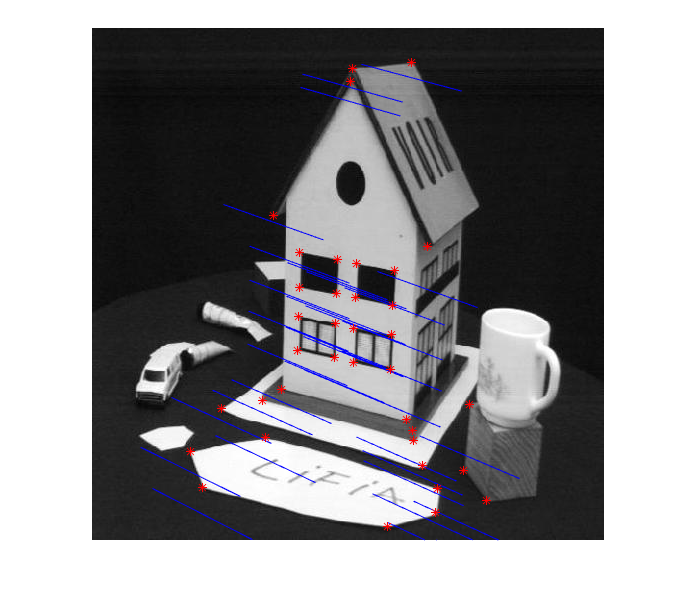
\includegraphics[scale=0.4]{wo1.png}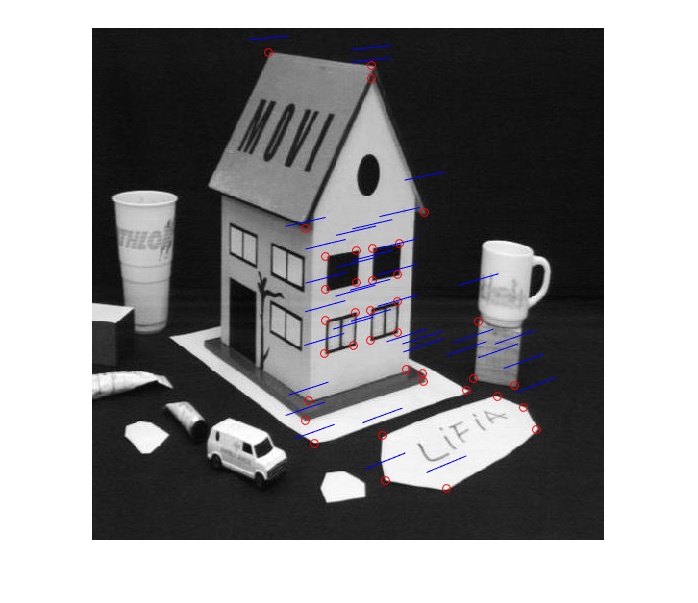
\includegraphics[scale=0.4]{wo2.png}
\end{figure}
For data set2, we have:
$$dis_{img1} = 9.7014,\quad dis_{img2} = 14.568$$
\begin{figure}[H]
	\centering
	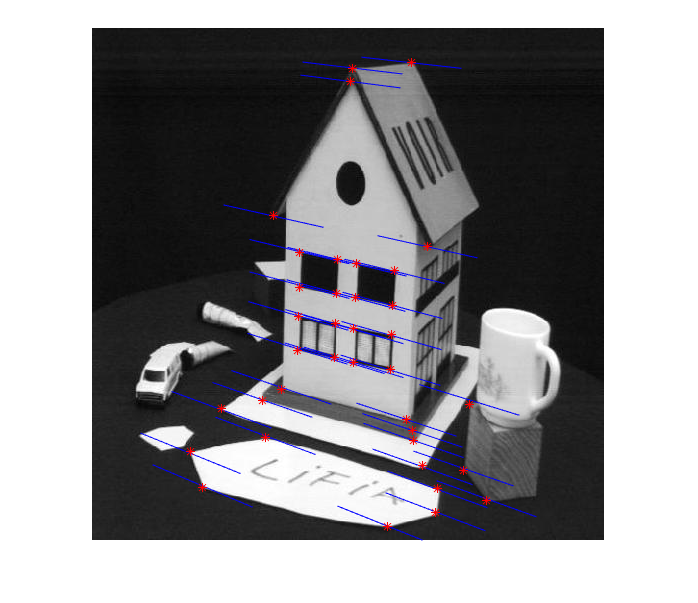
\includegraphics[scale=0.4]{wo3.png}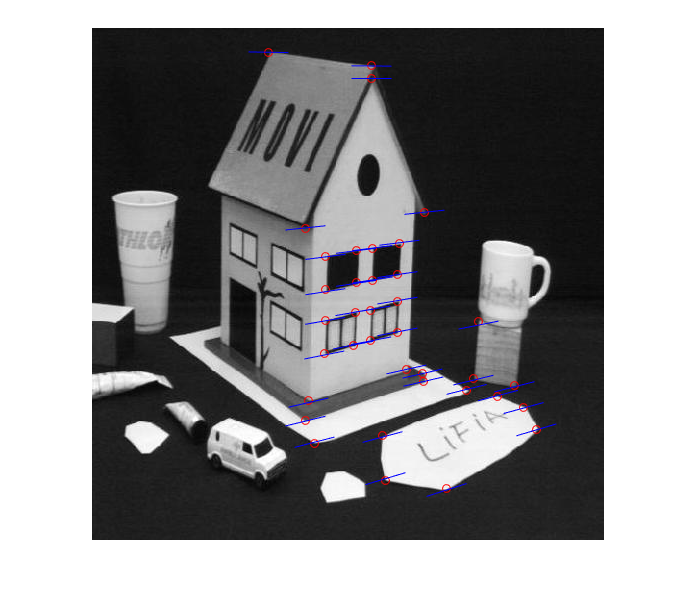
\includegraphics[scale=0.4]{wo4.png}
\end{figure}
Secondly, we apply 8 point logrithm with normalization:\\
For data set1, we have:
$$dis_{img1} = 0.8844,\quad dis_{img2} = 0.82422$$
\begin{figure}[H]
	\centering
	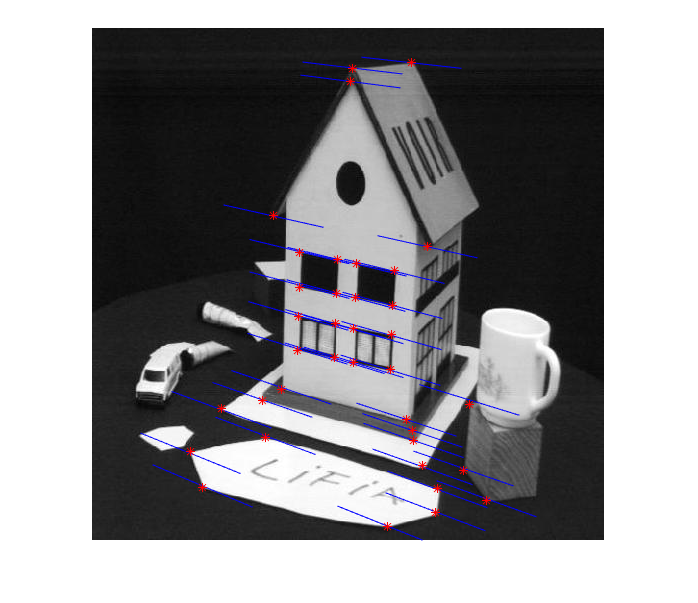
\includegraphics[scale=0.4]{r1.png}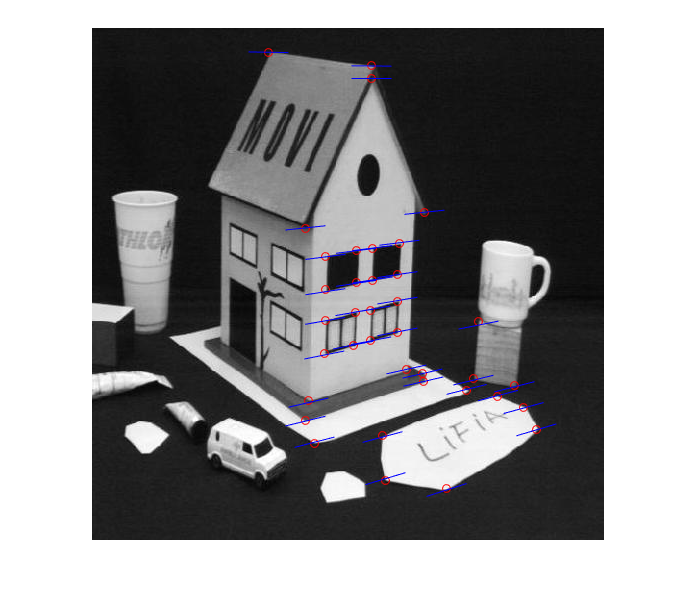
\includegraphics[scale=0.4]{r2.png}
\end{figure}
For data set2, we have:
$$dis_{img1} = 0.8914,\quad dis_{img2} = 0.89353$$
\begin{figure}[H]
	\centering
	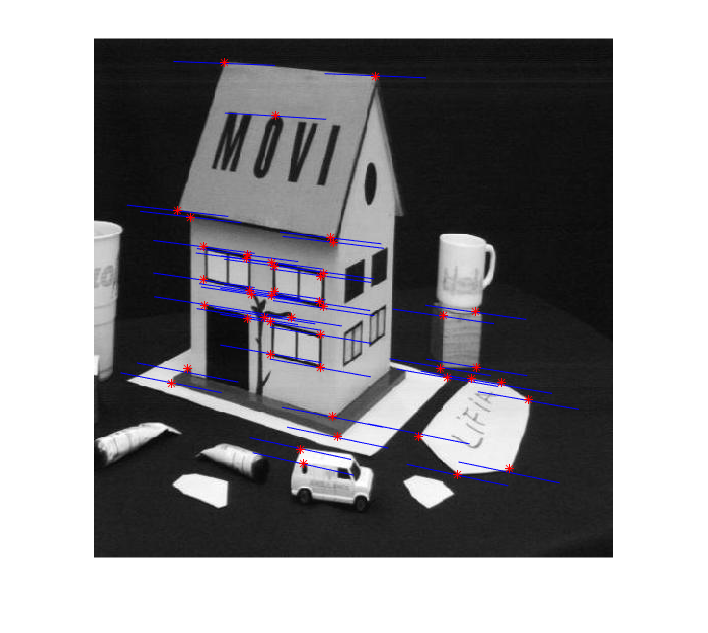
\includegraphics[scale=0.4]{r3.png}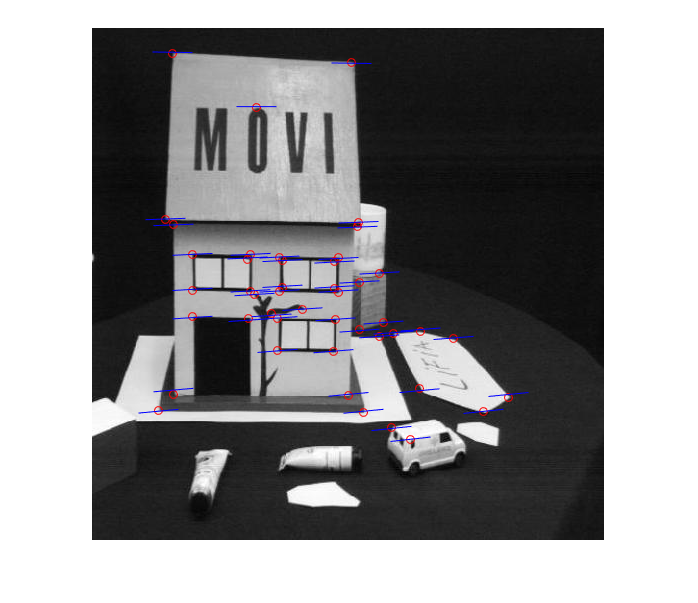
\includegraphics[scale=0.4]{r4.png}
\end{figure}
\subsection*{3.2 Stereo Rectification}
Stereo rectification, the results are shown below:\\
For set1,
$$H = 
\begin{bmatrix}
2.1065\times 10^{-6} & -1.647\times 10^{-6} & -3.354\times 10^{-6}\\
1.2335\times 10^{-6} & -5.9127\times 10^{-6} & -1.717\times 10^{-3}\\
-6.2663\times 10^{-9} & 2.013\times 10^{-1} & 1.0212\times 10^{-5}
\end{bmatrix}
$$
$$H' = 
\begin{bmatrix}
-9.9489\times 10^{-1} & -1.01\times 10^{-1} & -2.8055\times 10^{2}\\
1.01\times 10^{-1} & -9.9489\times 10^{-1} & -2.884\times 10^{2}\\
9.3144\times 10^{-4} & 9.4559\times 10^{-5} & 1.2627
\end{bmatrix}
$$
$$err = 74.279$$
For set2,
$$H = 
\begin{bmatrix}
-7.3225\times 10^{-7} & 2.7156\times 10^{-6} & 2.2629\times 10^{-3}\\
-5.4272\times 10^{-7} & 5.2278\times 10^{-6} & 1.4334\times 10^{-3}\\
2.2287\times 10^{-9} & -9.5275\times 10^{-11} & -7.5068\times 10^{-6}
 \end{bmatrix}
$$
$$H' = 
\begin{bmatrix}
-9.9279\times 10^{-1} & -1.1988\times 10^{-1} & -2.8484\times 10^{2}\\
1.1988\times 10^{-1} & -9.9279\times 10^{-1} & -2.2347\times 10^{-2}\\
5.8878\times 10^{-4} & 7.1092\times 10^{-5} & 1.1689 
\end{bmatrix}
$$
$$err = 58.188$$
Matlab codes are attached:
\lstinputlisting[firstline=1, lastline=100]{FMatrix.m}
\lstinputlisting[firstline=1, lastline=100]{FMatrix_normalization.m}
\lstinputlisting[firstline=1, lastline=100]{imageRect.m}
\end{document}